\documentclass{assets/utmreport}

\usepackage{booktabs,amssymb,float,graphicx,listings}

\hypersetup{hidelinks,hypertexnames=false,pdfauthor={Lucian-Adrian Gavril}}

\selectlanguage{english}

\utmlogo{assets/utm-logo.jpeg}

\institution{Technical University of Moldova}
\faculty{Faculty of Computers, Informatics, and Microelectronics}
\department{Department of Software Engineering}
\studyprogramme{Software Engineering Study Programme}
\documenttype{Laboratory report}
\reporttitle{Operating Systems Laboratory 8}
\reportsubtitle{The Same Calls Inside Your Own OS}
\student{Lucian-Adrian Gavril}{FAF-241}
\supervisor{Reițman Patricia}{univ. assist.}
\cityyear{Chișinău}{2026}

\setlength{\emergencystretch}{3em}
\lstset{basicstyle=\ttfamily\fontsize{10}{12}\selectfont,breaklines=true,columns=fullflexible,keepspaces=true,showstringspaces=false,numbers=left,numberstyle=\tiny\color{gray},frame=single,rulecolor=\color{gray},tabsize=2}

\begin{document}
\makeutmreporttitlepage
\tableofcontents
\clearpage
\begin{utmabstract}[Abstract]
This laboratory repeats process creation, program replacement and waiting inside xv6, then implements a one-byte request and reply using two pipes. The report compares the xv6 and Linux interfaces, traces the kernel boundary and explains descriptor ownership. A clean build and QEMU boot demonstrate echo, the successful and failed exec variants, ordered ping-pong output and an optional process chain filtering primes from 2 through 35.
\utmkeywords{processes, system calls, file descriptors, pipes, linux, xv6}
\end{utmabstract}
\utmintroduction
The required experiments follow the laboratory handout\cite{brief}; the process and descriptor model follows the course lecture\cite{lecture}. The supplied source is reproduced in Appendix A. A successful execution is evidence for that captured environment, while the concept figures explain the general mechanism.

The UNIX process interface lets a shell compose small programs without changing their implementations. Process calls control which program runs and when its completion is collected; file descriptors select where the program reads and writes. These mechanisms explain redirection, pipelines and communication between processes.
The required \texttt{run} program demonstrates \texttt{fork}, \texttt{exec} and \texttt{wait}; user/pingpong.c demonstrates a one-byte exchange over two pipes. The QEMU observations below record the behavior of these programs in xv6.


\chapter{Processes and \texttt{exec}}
Figure~\ref{fig:lifetime} distinguishes a new process from a replacement program. The amber interval represents an exited child retained until its parent reaps it; the child executes no instructions in that interval.

\begin{figure}[htbp]
\centering
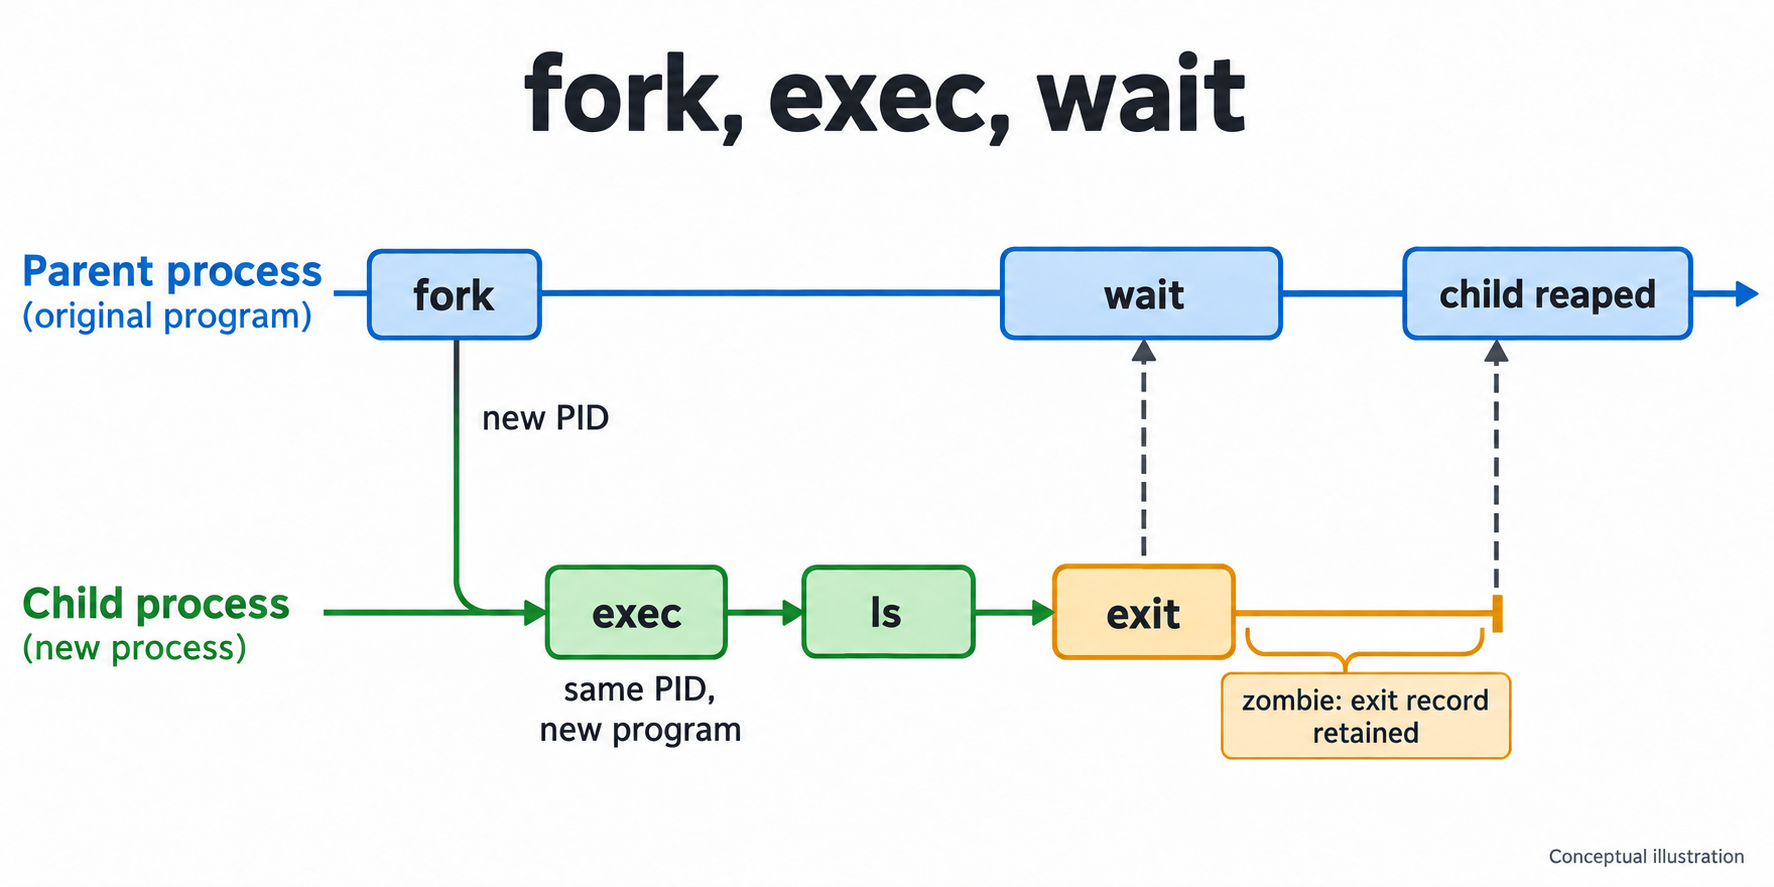
\includegraphics[width=\textwidth]{assets/concept-process-lifetime.png}
\caption{Process lifetime and the retained exit record. ImageGen concept illustration, 23 October 2026; scheduling is schematic.}
\label{fig:lifetime}
\end{figure}


The xv6 process interface is small enough to trace through its source. \texttt{user/usys.pl} generates wrappers that place the system-call number in register \texttt{a7} and execute \texttt{ecall}. The trap path enters \texttt{usertrap}; \texttt{kernel/syscall.c} dispatches the request. Process creation and waiting are implemented in \texttt{kernel/proc.c}; \texttt{kernel/exec.c} constructs the replacement user image\cite{xv6}.

In \texttt{user/run.c}, the child passes an argument vector to \texttt{exec("echo", args)}. The vector contains the executable name, four argument words and a null terminator. The loaded \texttt{echo} program prints the argument words. The parent's later wait obtains completion information rather than the child's text output.


\begin{figure}[htbp]
\centering
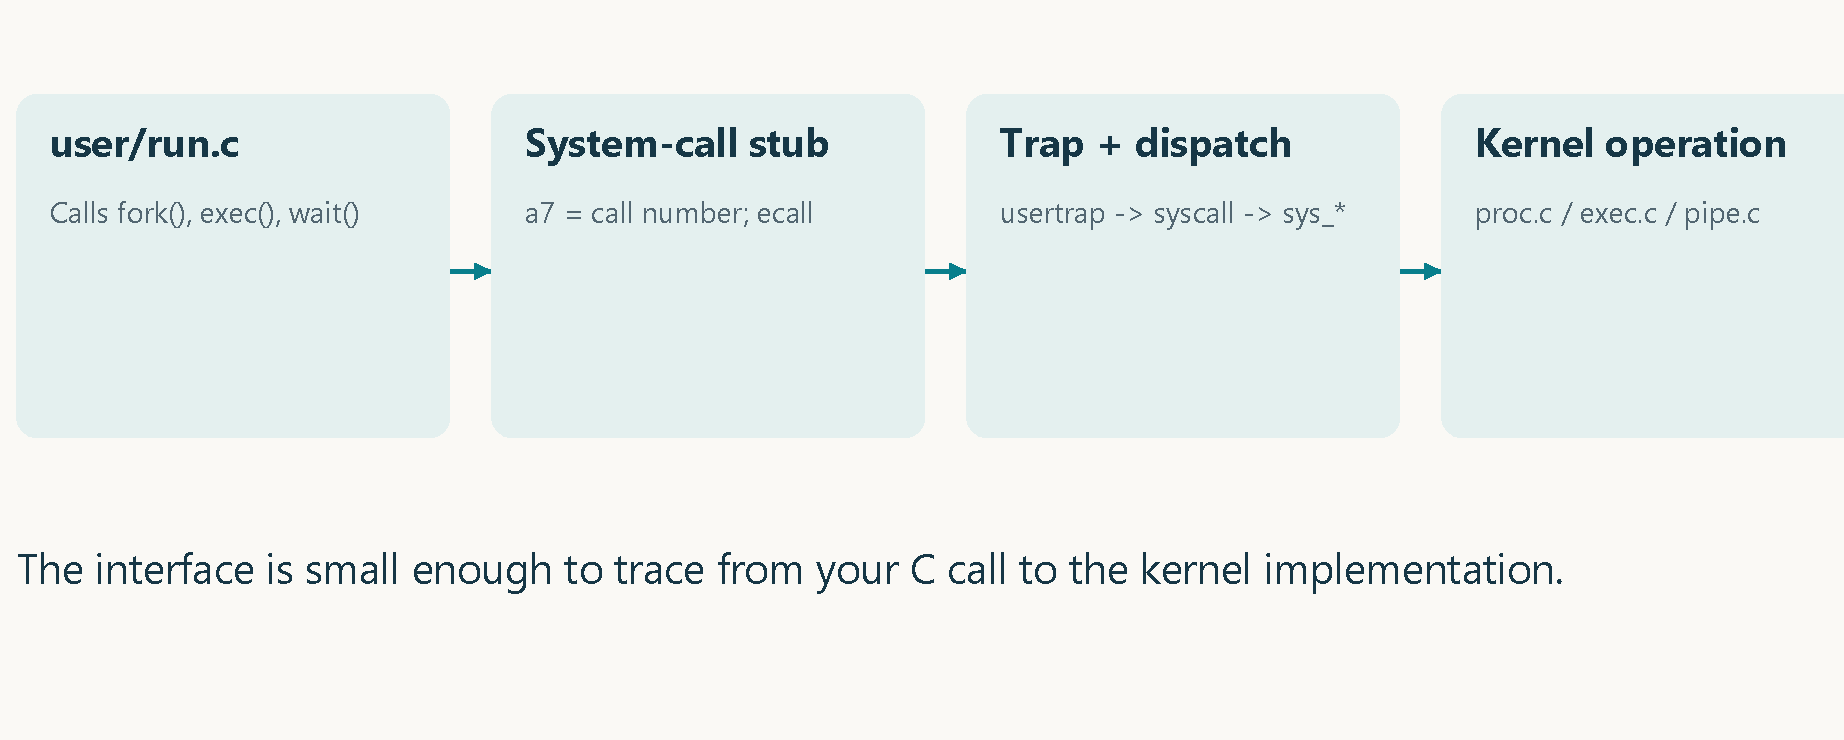
\includegraphics[width=\textwidth]{assets/xv6-call-path.pdf}
\caption{The user-call stub enters the kernel through ecall; the dispatcher selects the requested kernel operation.}
\end{figure}


\begin{enumerate}

\item xv6 and Linux use the same basic sequence: \texttt{fork} creates a child process, \texttt{exec} replaces the child's program image, and the parent calls a wait operation to collect the child's completion. The APIs differ. xv6 provides \texttt{exec(path,\allowbreak{} argv)} and \texttt{wait(\&status)}; Linux commonly uses \texttt{execlp} and \texttt{waitpid}. \texttt{execlp} searches \texttt{PATH}, while xv6 \texttt{exec} is passed a path directly. Linux's wait status is encoded and normally decoded with macros such as \texttt{WEXITSTATUS}; this xv6 implementation copies the child's integer exit value to \texttt{status};

\item The child process prints \texttt{child pid} before the call to \texttt{exec}. If \texttt{exec} succeeds, that child becomes the \texttt{echo} program. The \texttt{echo} program prints \texttt{hello from the child}. The parent remains in \texttt{run} and prints the child's PID and status only after \texttt{wait} returns;

\item The missing-program variant prints \texttt{exec failed} and explicitly calls \texttt{exit(1)}, so xv6's \texttt{wait(\&status)} reports status 1. In Lab 7's Linux \texttt{run.\allowbreak{}c}, the \texttt{execlp} failure branch instead calls \texttt{exit(127)}, and the parent decodes 127 with \texttt{WEXITSTATUS(status)}. Both values are chosen by the child program's error branch; a failed \texttt{exec} call does not itself choose an exit status. Shells also commonly use 127 for a command they cannot find;

\end{enumerate}


\begin{figure}[H]
\centering
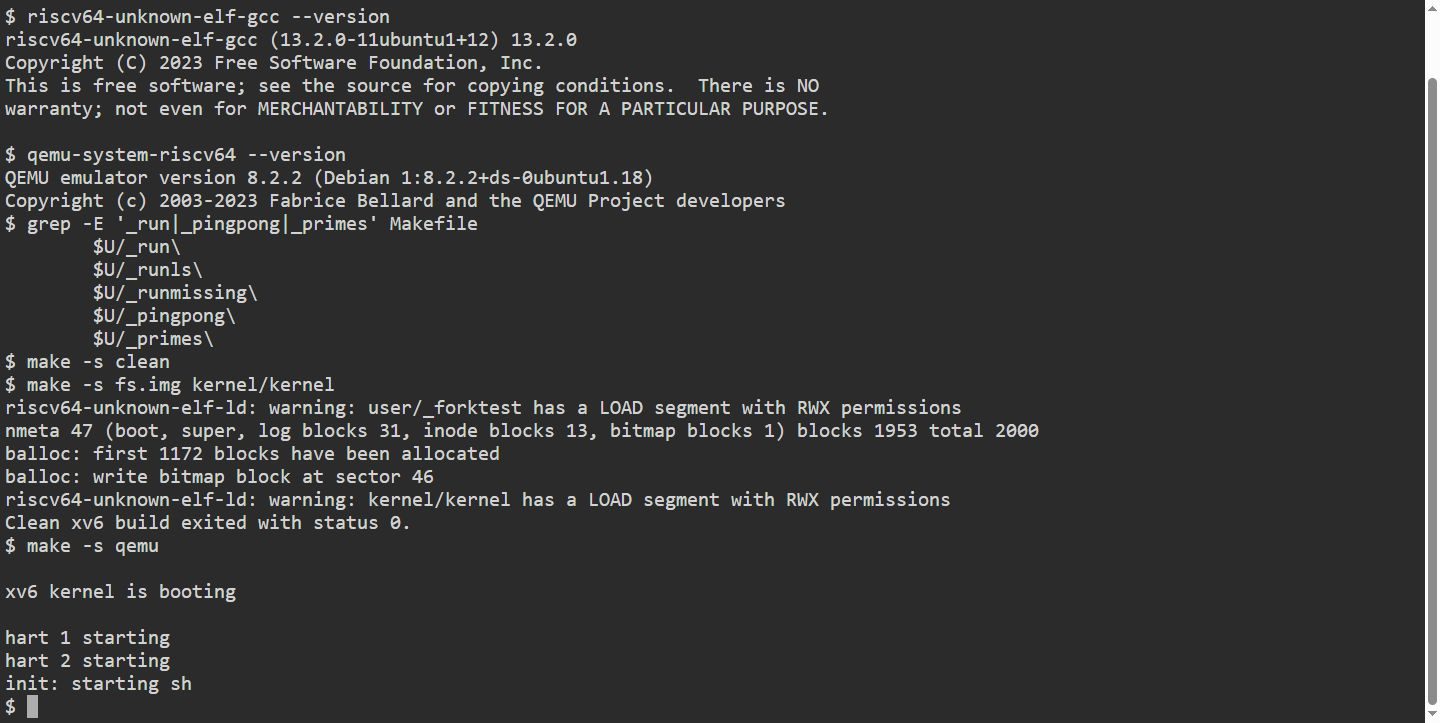
\includegraphics[trim=0bp 0.00bp 320.00bp 0bp,clip,width=\textwidth,height=0.72\textheight,keepaspectratio]{assets/proof-build-boot.png}
\caption{Clean xv6 build, required UPROGS entries, tool versions and successful QEMU boot. Live ttyd terminal capture, 19 October 2026. Only blank margins are cropped in this report; program output is unchanged.}
\end{figure}


\begin{figure}[H]
\centering
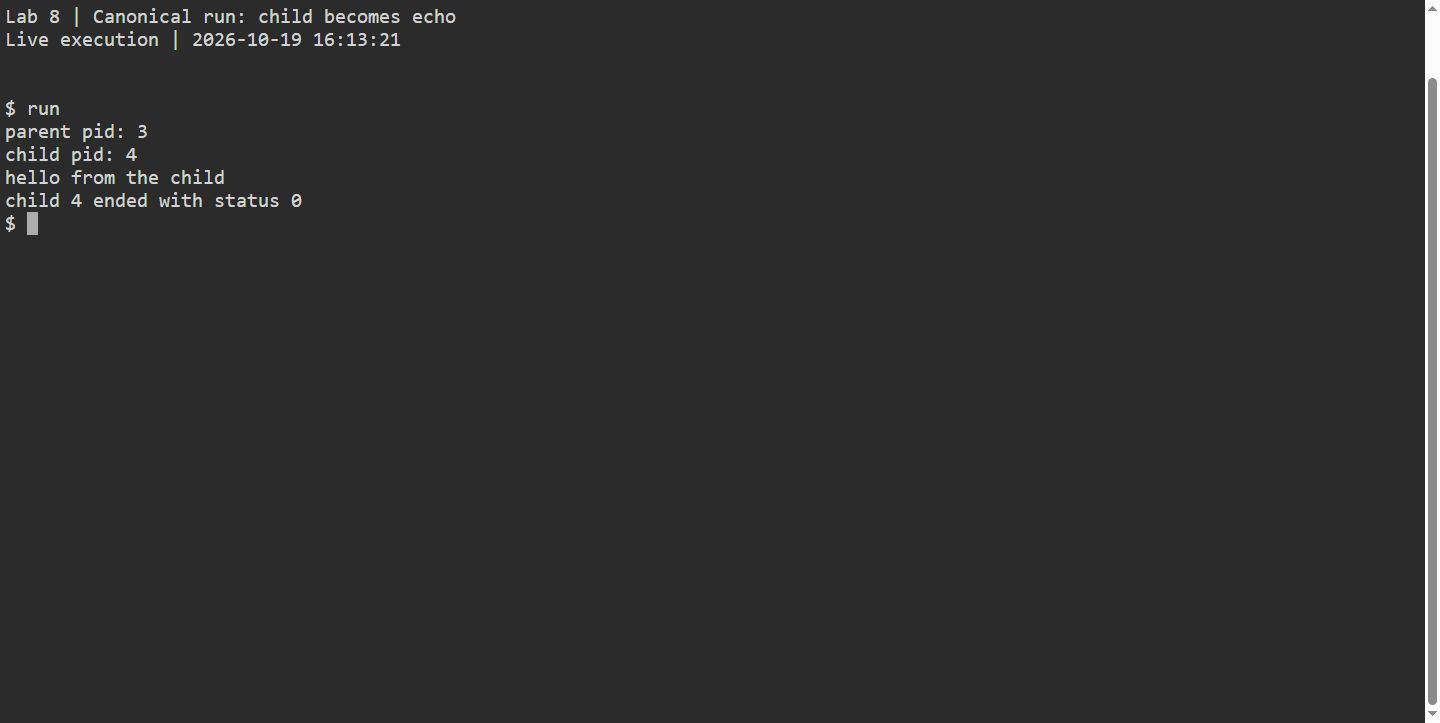
\includegraphics[trim=0bp 470.00bp 320.00bp 0bp,clip,width=\textwidth,height=0.72\textheight,keepaspectratio]{assets/proof-run-echo.png}
\caption{The canonical run program starts an echo child and collects exit status 0. Live ttyd terminal capture, 19 October 2026. Only blank margins are cropped in this report; program output is unchanged.}
\end{figure}


\chapter{\texttt{exec} variants}

Changing only the argument array and target tests a successful \texttt{ls} replacement and a failed \texttt{nosuchprog} replacement. The saved \texttt{user/\allowbreak{}run.\allowbreak{}c} remains the required echo example. In the missing-program case, \texttt{exec} returns an error, so the child reaches the diagnostic and \texttt{exit(1)}. For \texttt{ls}, successful \texttt{exec} never returns to \texttt{run}'s child branch.



\begin{figure}[H]
\centering
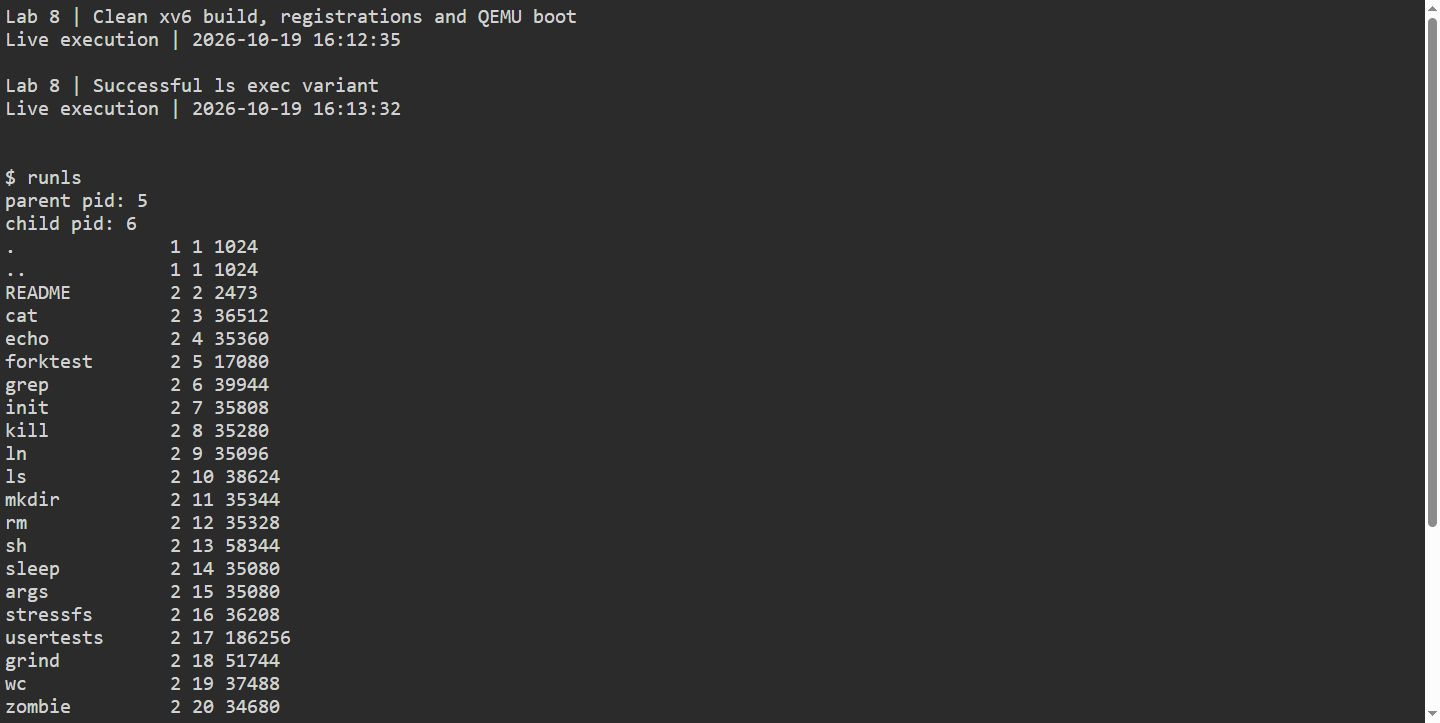
\includegraphics[trim=0bp 0.00bp 320.00bp 0bp,clip,width=\textwidth,height=0.72\textheight,keepaspectratio]{assets/proof-run-ls-start.png}
\caption{The overlay-only runls command starts parent 5 and child 6, which executes ls; the listing begins here. Live ttyd terminal capture, 19 October 2026. Only blank margins are cropped in this report; program output is unchanged.}
\end{figure}


\begin{figure}[H]
\centering
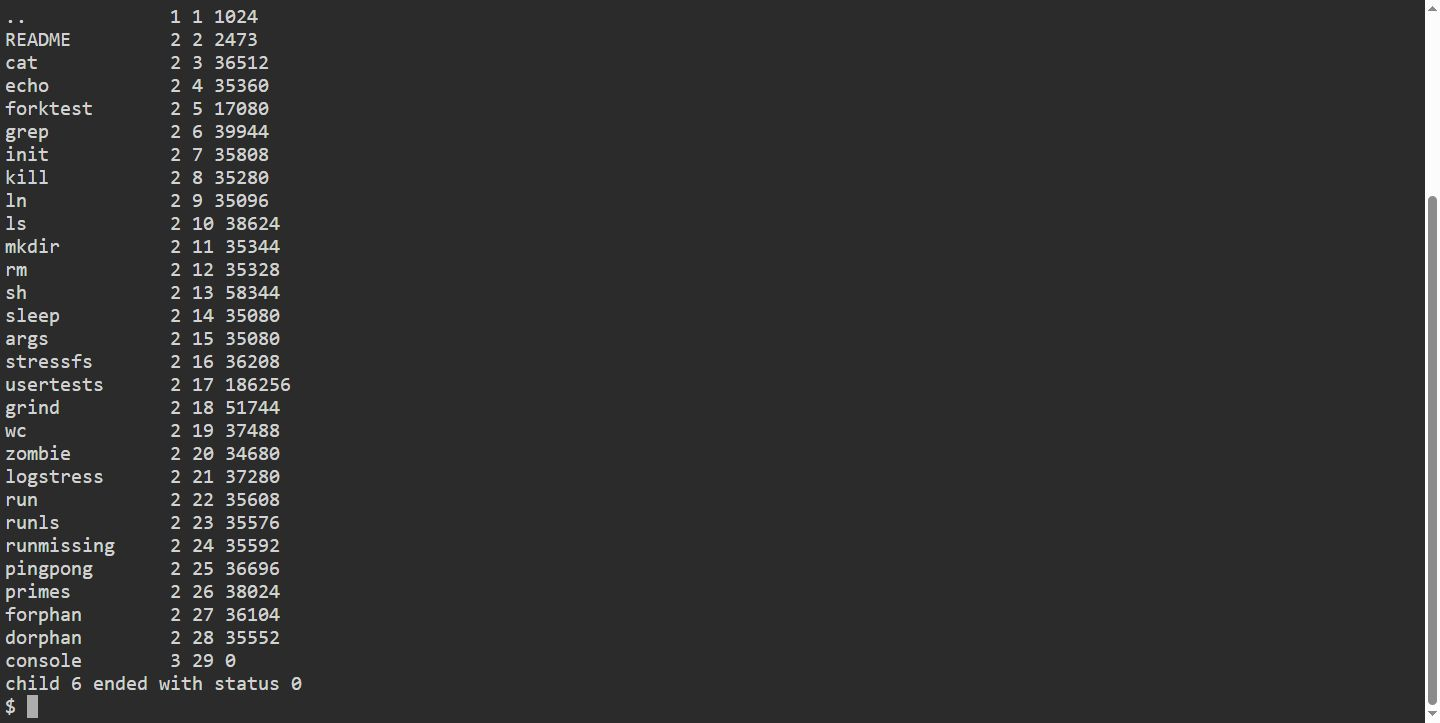
\includegraphics[trim=0bp 0.00bp 320.00bp 0bp,clip,width=\textwidth,height=0.72\textheight,keepaspectratio]{assets/proof-run-ls.png}
\caption{Continuation of the same ls variant: the listing finishes and the parent collects child 6 with status 0. Live ttyd terminal capture, 19 October 2026. Only blank margins are cropped in this report; program output is unchanged.}
\end{figure}


\begin{figure}[H]
\centering
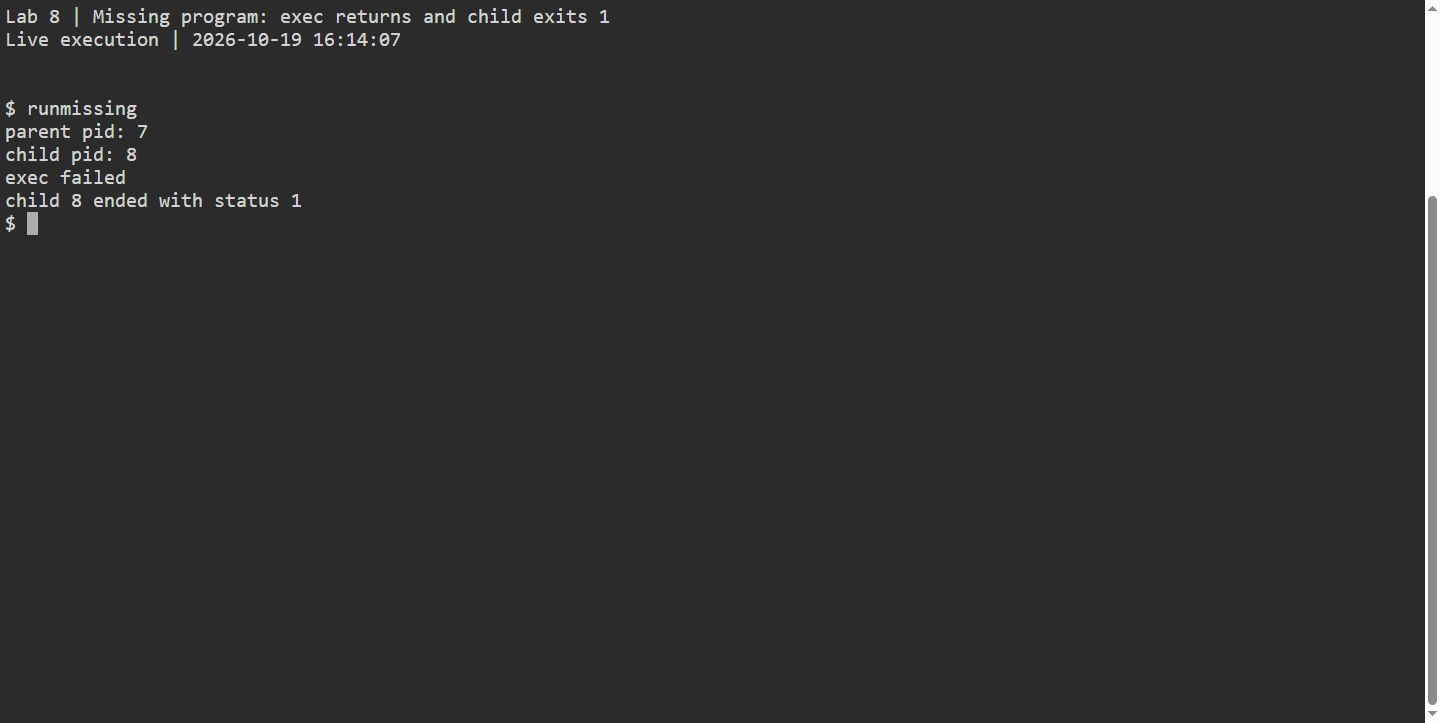
\includegraphics[trim=0bp 470.00bp 320.00bp 0bp,clip,width=\textwidth,height=0.72\textheight,keepaspectratio]{assets/proof-run-missing.png}
\caption{The missing-program variant reaches exec failed and the explicit exit(1) branch. Live ttyd terminal capture, 19 October 2026. Only blank margins are cropped in this report; program output is unchanged.}
\end{figure}


\chapter{Two pipes}
Figure~\ref{fig:pipe-eof} shows why closing unused endpoints is part of the algorithm. The two-direction xv6 exchange applies this rule independently to each pipe.

\begin{figure}[htbp]
\centering
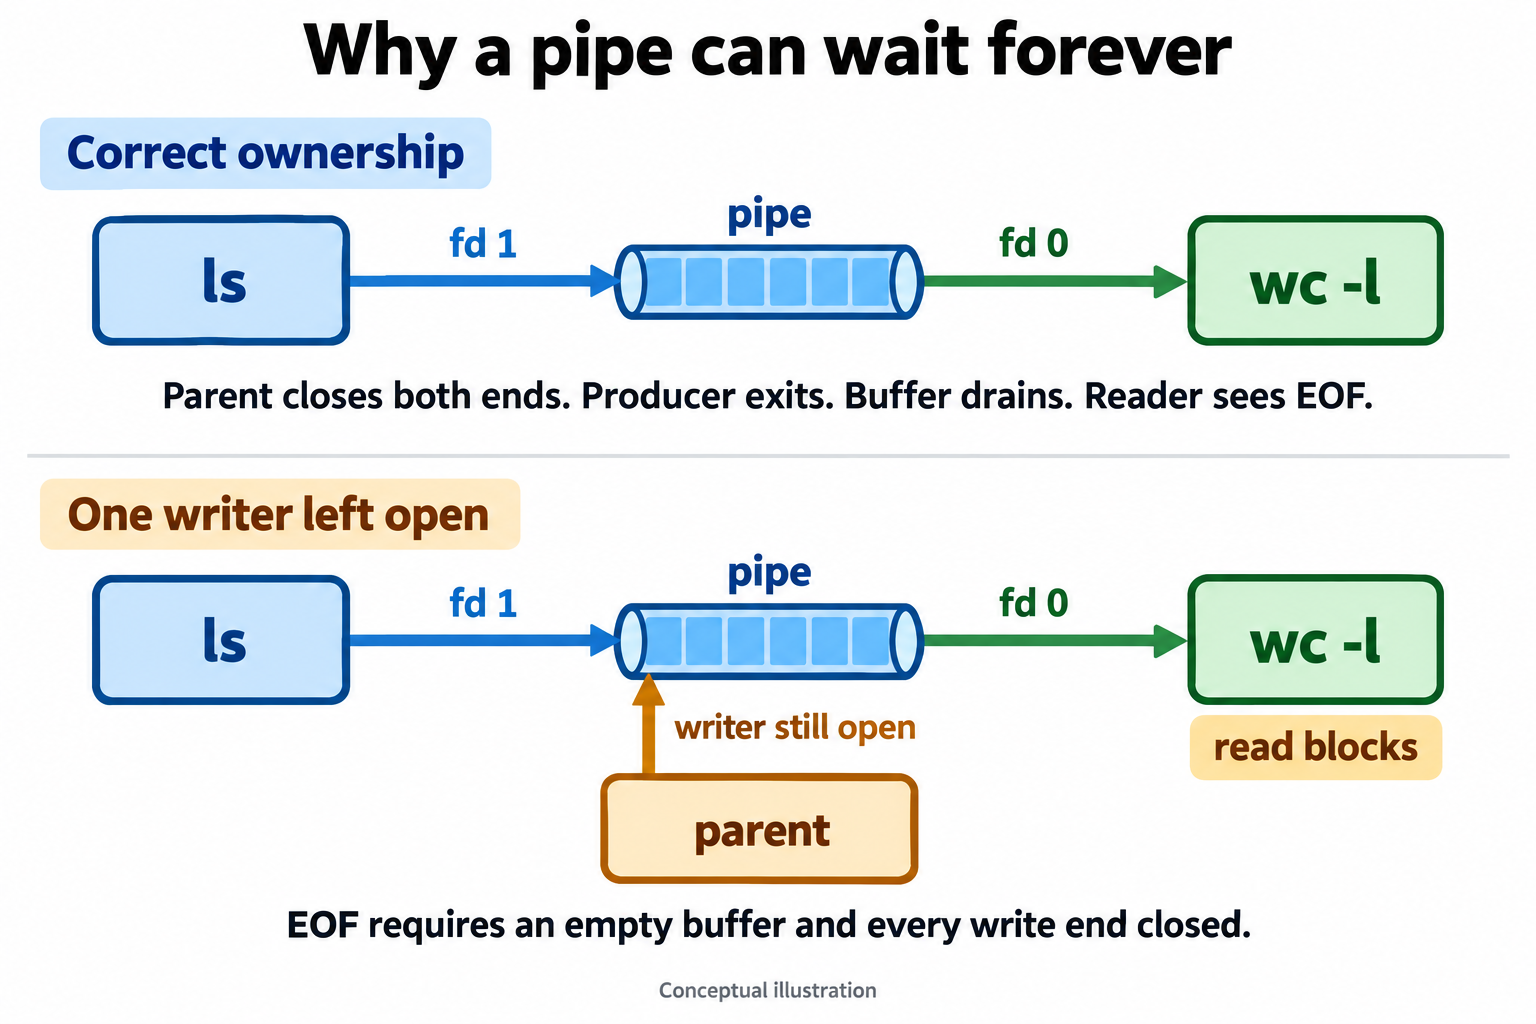
\includegraphics[width=\textwidth]{assets/concept-pipe-ownership.png}
\caption{Writer ownership determines end-of-file. ImageGen concept illustration, 23 October 2026; not measured output.}
\label{fig:pipe-eof}
\end{figure}


The pipes are created before the fork so both processes inherit their endpoints. \texttt{parent\_to\_child} carries the request; \texttt{child\_to\_parent} carries the reply. The parent initializes a one-byte token. Every read and write checks that one byte was transferred. The two streams give each direction a separate reader, avoiding a race in which a process could read its own message from one shared pipe.


\begin{figure}[htbp]
\centering
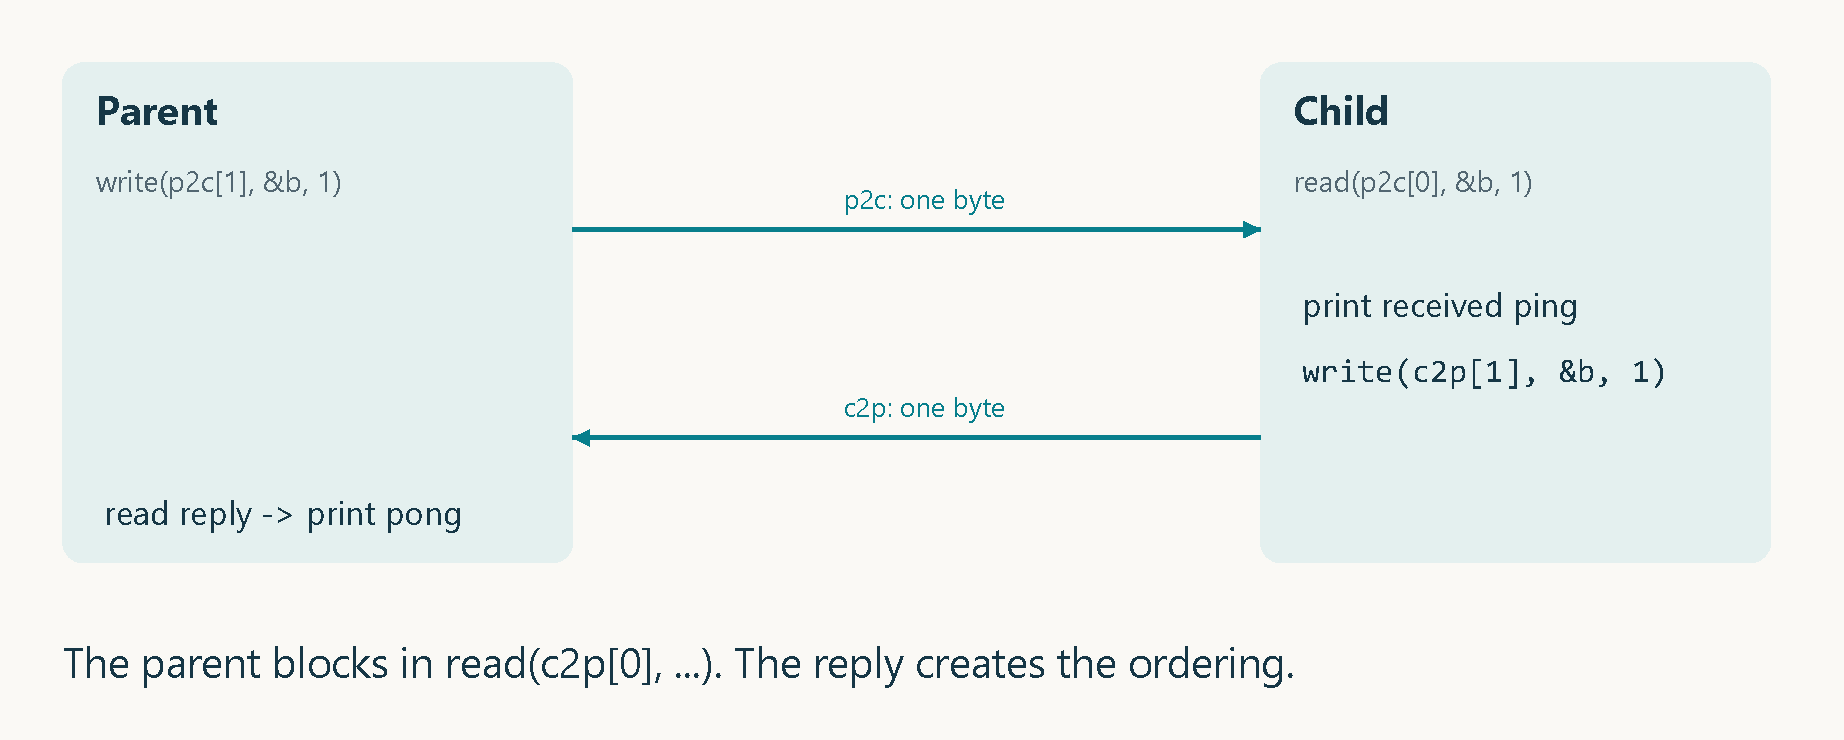
\includegraphics[width=\textwidth]{assets/pingpong-exchange.pdf}
\caption{A request byte travels parent to child; its reply travels child to parent on a separate pipe.}
\end{figure}


The parent writes the ping byte to \texttt{parent\_\allowbreak{}to\_\allowbreak{}child[1]}; the child reads it from \texttt{parent\_\allowbreak{}to\_\allowbreak{}child[0]}. The child writes the pong byte to \texttt{child\_\allowbreak{}to\_\allowbreak{}parent[1]}; the parent reads it from \texttt{child\_\allowbreak{}to\_\allowbreak{}parent[0]}. xv6 pipes are one-way streams, so the two directions use separate pipes. With one shared pipe, both processes would read and write through the same stream, and a reader could consume the byte it had just written.


The parent blocks in \texttt{read(child\_\allowbreak{}to\_\allowbreak{}parent[0],\allowbreak{} .\allowbreak{}.\allowbreak{}.\allowbreak{})} until the child writes its reply. \texttt{wait(0)} comes after the reply and collects the child's exit; it is not the call that waits for the pong byte. Each process closes the ends it does not use. That makes the ownership of each direction explicit and allows EOF to reach a reader when the remaining writers close.



\begin{figure}[H]
\centering
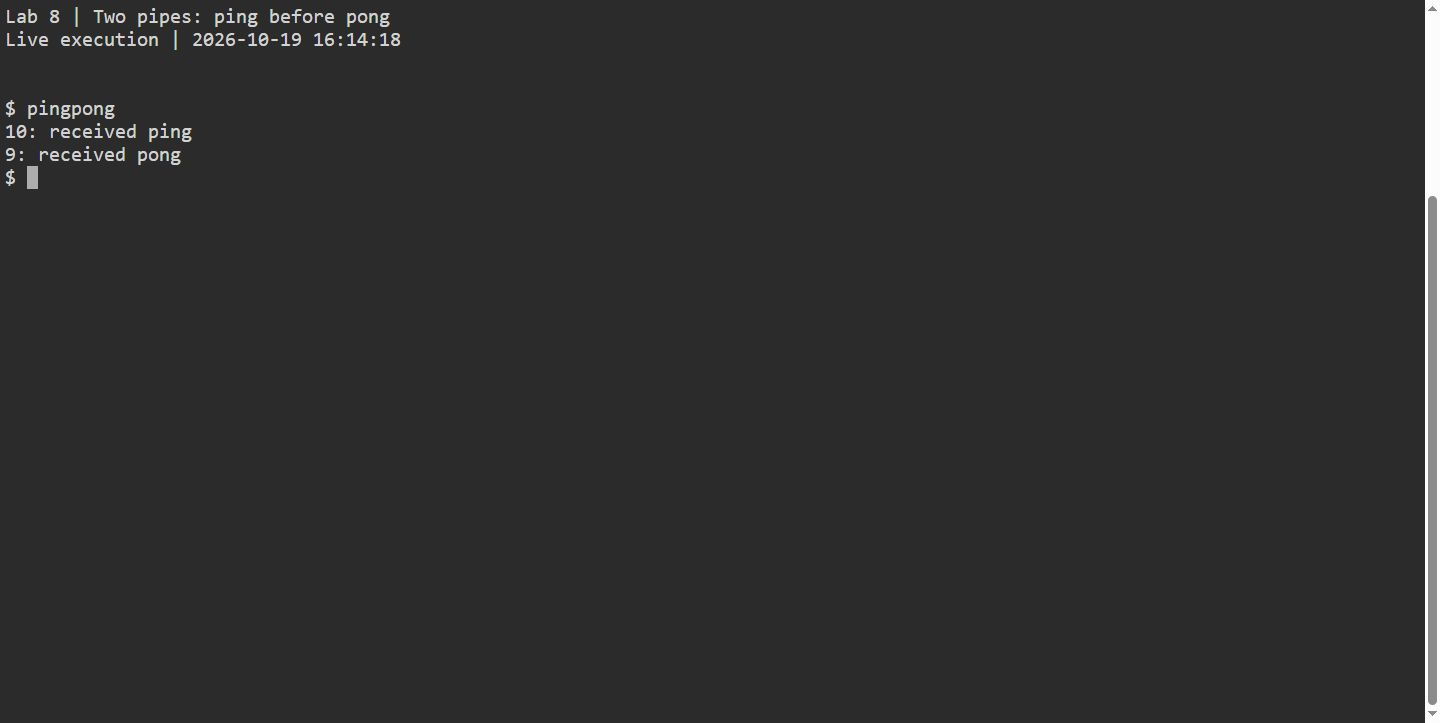
\includegraphics[trim=0bp 516.00bp 320.00bp 0bp,clip,width=\textwidth,height=0.72\textheight,keepaspectratio]{assets/proof-pingpong.png}
\caption{Actual xv6 execution: the child prints received ping before the parent prints received pong. Live ttyd terminal capture, 19 October 2026. Only blank margins are cropped in this report; program output is unchanged.}
\end{figure}


\chapter{QEMU observations}

The programs build cleanly with RISC-V GCC 13.2.0 and boot under QEMU 8.2.2. The captured console output and invocation are in the fresh capture transcript. The successful run uses a disposable Lab 2 overlay and the Makefile's default three CPUs.


Observed in that QEMU session:


\begin{lstlisting}

$ run

parent pid: 3

child pid: 4

hello from the child

child 4 ended with status 0



$ pingpong

10: received ping

9: received pong



$ primes

prime 2

prime 3

prime 5

prime 7

prime 11

prime 13

prime 17

prime 19

prime 23

prime 29

prime 31

\end{lstlisting}

For the successful \texttt{ls} variant, an overlay-only build printed the xv6 root-directory entries and the parent observed child status 0. For the missing-program variant, an overlay-only build printed \texttt{exec failed}, and the parent observed child status 1. Those two temporary executables were generated from \texttt{run.\allowbreak{}c} by changing only its argument array and \texttt{exec} target; the submitted source remains the echo example. Process IDs depend on the boot and are recorded here only for this run.



\begin{figure}[H]
\centering
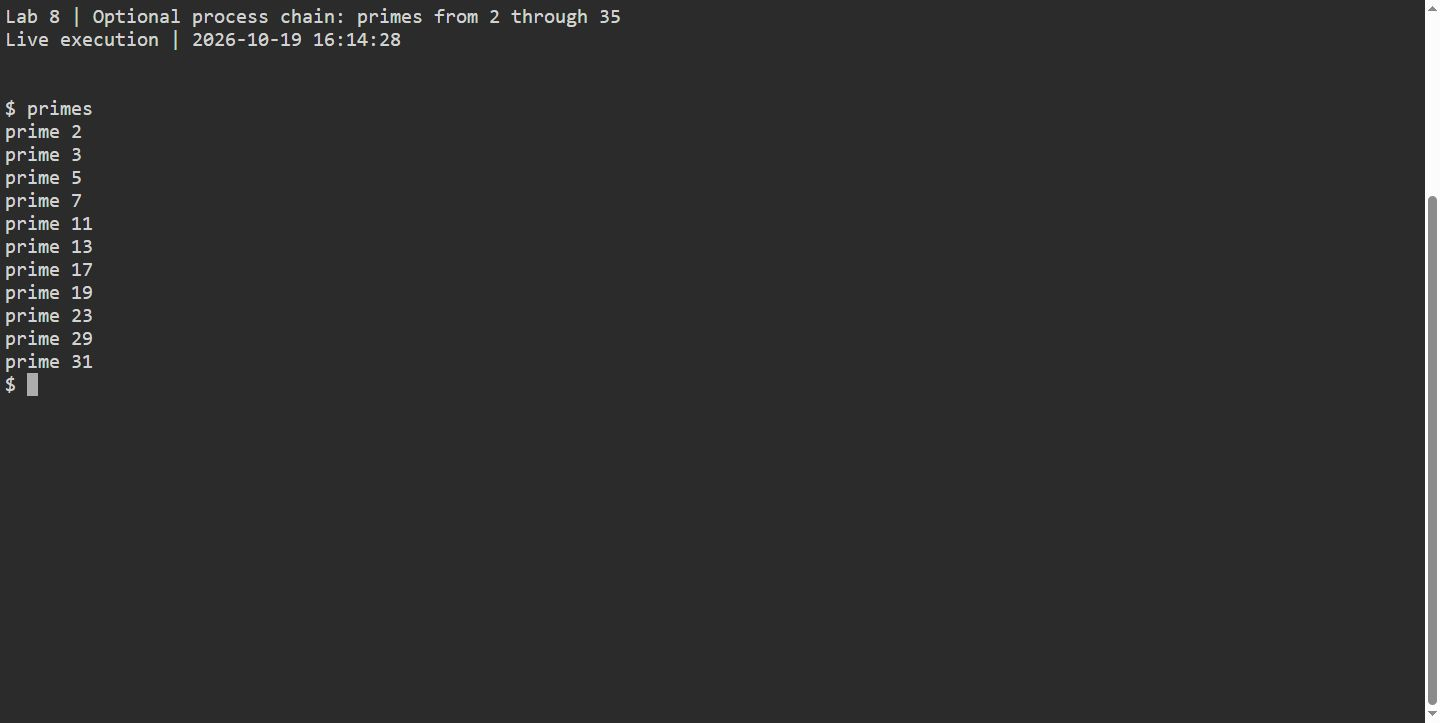
\includegraphics[trim=0bp 309.00bp 320.00bp 0bp,clip,width=\textwidth,height=0.72\textheight,keepaspectratio]{assets/proof-primes.png}
\caption{The optional process chain prints exactly the primes from 2 through 35. Live ttyd terminal capture, 19 October 2026. Only blank margins are cropped in this report; program output is unchanged.}
\end{figure}
\chapter{Optional prime-filter chain}
The producer sends the integers 2 through 35. Each stage reads its first surviving number as a prime, prints it and passes only numbers not divisible by that prime to a new child stage. Earlier stages have already removed multiples of smaller primes. Every stage closes its output when its input ends, allowing EOF to propagate, and waits for the child it created. The observed eleven outputs are listed in the QEMU results.

\begin{figure}[htbp]
\centering
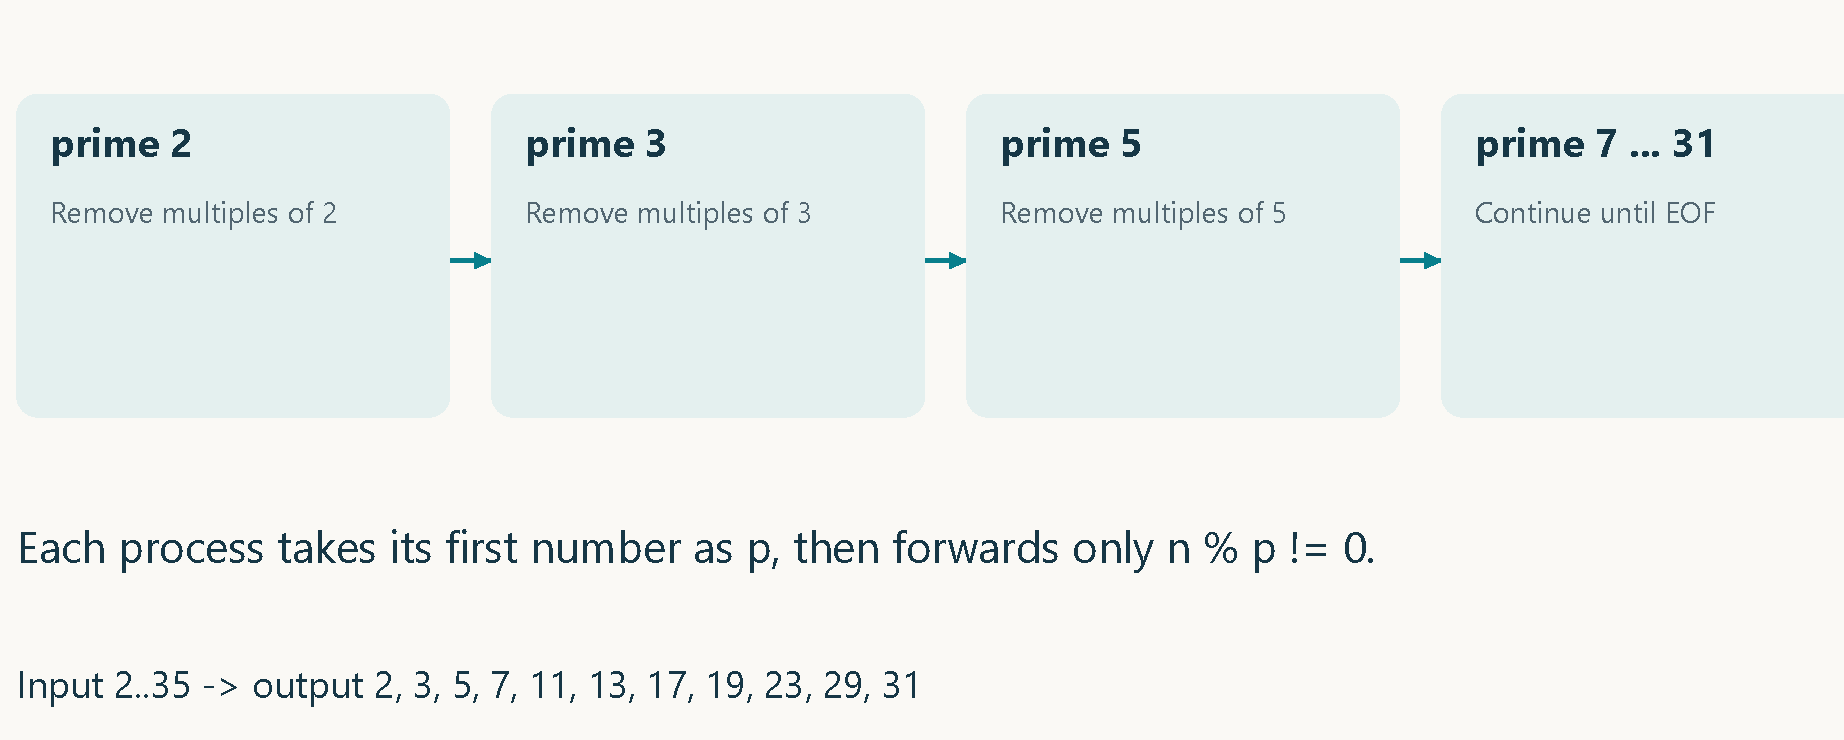
\includegraphics[width=\textwidth]{assets/prime-filter-chain.pdf}
\caption{Each process removes multiples of one prime and forwards the remaining integers.}
\end{figure}

\begin{figure}[htbp]
\centering
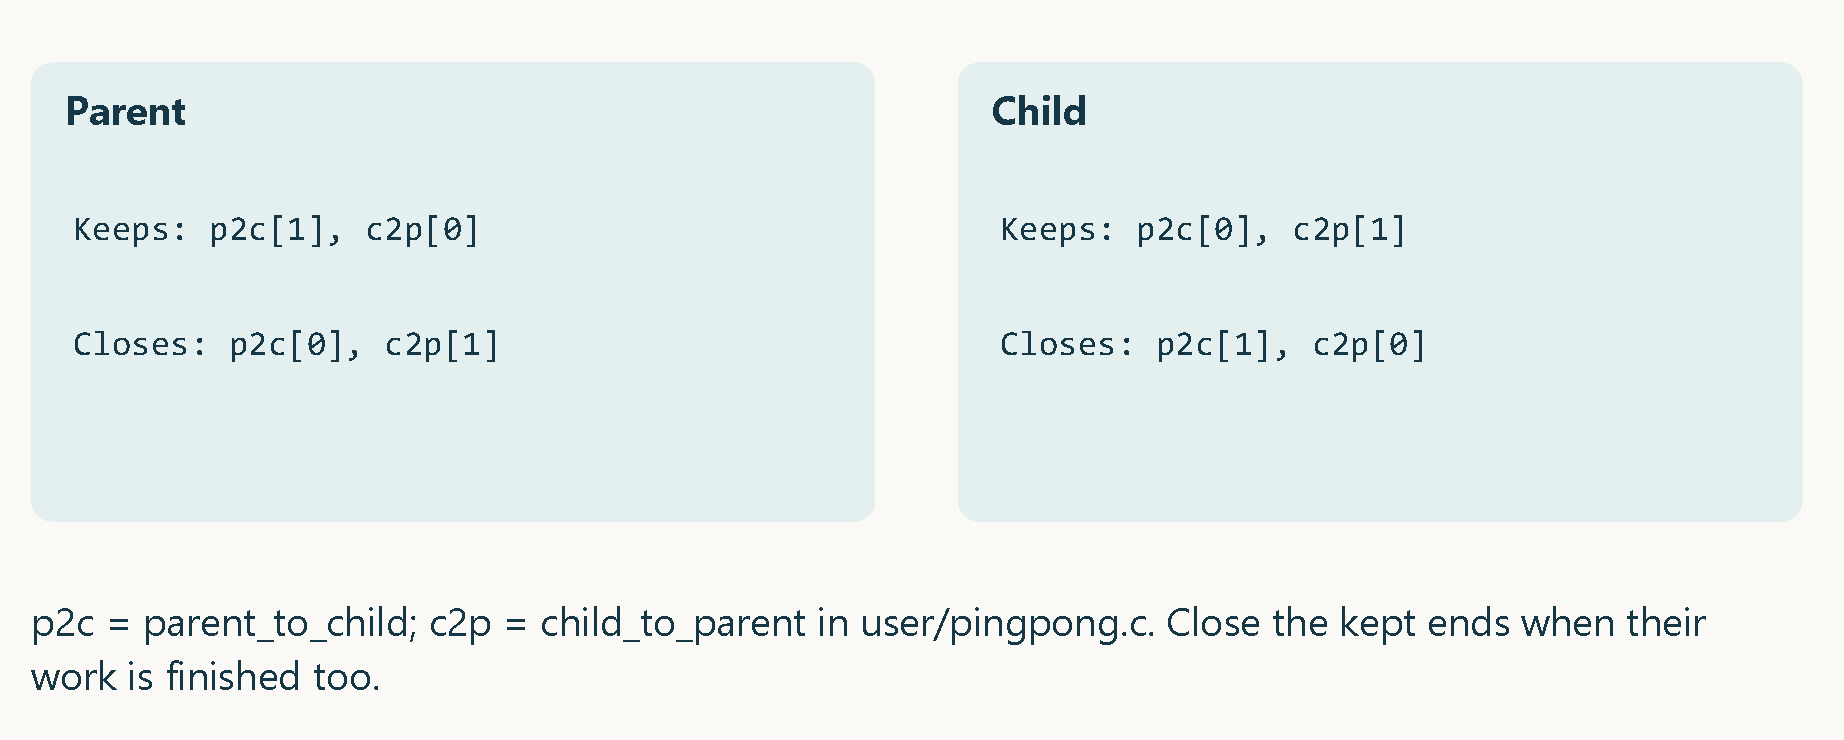
\includegraphics[width=\textwidth]{assets/pipe-ownership.pdf}
\caption{After fork, each process closes the endpoint copies it does not use, then closes its used ends after the exchange.}
\end{figure}
\utmconclusions
The xv6 run demonstrates the same process lifecycle as the Linux example while exposing its kernel implementation. The echo and ls children exited successfully; the explicit failed-exec branch returned status 1. Two pipes made the ping and reply directions independent. Blocking read enforced ping-before-pong ordering, and the later wait reaped the child. The optional filter chain demonstrated the same ownership and EOF rules across multiple stages.
\begin{thebibliography}{9}
\bibitem{brief} Operating Systems, FCIM/FAF, UTM. \textit{Laboratory 8 handout}, academic year 2026--2027. Accessed 19 October 2026. \url{https://else.fcim.utm.md/mod/resource/view.php?id=72240}.
\bibitem{lecture} Operating Systems. \textit{Processes, Descriptors, Pipes}, Session 4. Accessed 19 October 2026. \url{https://else.fcim.utm.md/mod/resource/view.php?id=72236}.
\bibitem{xv6} MIT. \textit{xv6-riscv source code}. Course source inspected 19 October 2026. Local course snapshot: \texttt{os/lab2}; \texttt{kernel/proc.c}, \texttt{kernel/exec.c}, \texttt{kernel/pipe.c} and \texttt{user/sh.c}.
\end{thebibliography}
\appendix
\chapter{Program source}
The following listings are the submitted programs. They accompany the observations in the main report.


\section{user/run.c}
\lstinputlisting[language=C]{user/run.c}

\section{user/pingpong.c}
\lstinputlisting[language=C]{user/pingpong.c}

\section{user/primes.c}
\lstinputlisting[language=C]{user/primes.c}

\end{document}
